\section{Bluetooth Architecture}
The Bluetooth technology is divided into two specifications: the core and the profile specifications. The core specification defines how the technology works, while the profiles define how to leverage on the core technologies to build a Bluetooth application.
The Bluetooth core system consists of an RF transceiver, the baseband, and a set of protocols.

\begin{figure}[ht!]
  \centering
  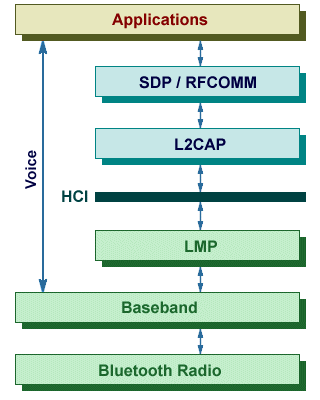
\includegraphics[width=0.3\textwidth]{img/bluetooth_protocol_stack.png} 
  \caption{Bluetooth protocol stack}
  \label{img:bt-protocol-stack}
\end{figure}

\subsection{L2CAP}
The L2CAP (Logical Link Control and Adaptation Layer) layer provides both connectionless and connection-oriented services to higher level protocols. Its tasks include multiplexing of protocols (since Baseband does not contemplate a "type" field to specify the kind of protocol that generated a package), segmentation and reassembly of PDUs (Protocol Data Unit), and QoS (Quality of Service) support.
L2CAP enables higher level applications and protocols to send and receive L2CAP data packets up to 64 kilobytes in length.

The L2CAP layer provides logical channels, named L2CAP channels, which act as a logical connection on top of a baseband connection.
More channels can rely on the same baseband connection.
An endpoint of an L2CAP channel is identified by a channel identifier (CID).

By default, L2CAP uses ACL as the transmission link.

\subsubsection{ACL}
Bluetooth supports two main types of connection links: ACL (Asynchronous Connection Less) and SCO (Synchronous Connection Oriented).
The most widely used one is ACL, which garantees that data is delivered and in the correct order and without errors.

ACL links can operate both in a symmetric and in a asymmetric mode, and can be granted a Quality of Service by setting the appropriate channel parameters during connection.

\subsection{RFCOMM}
The RFCOMM protocol emulates the capabilities of the RS-232 serial ports over the L2CAP protocol. It was developed to make it easier for manufacterers to use the Bluetooth technology in their existing applications. Similarly to TCP, RFCOMM provides applications a simple point-to-point reliable data stream, supporting multiplexing and flow control between devices and applications.

It is possible to maintain up to 60 simultaneous connections between two devices (each one can initialize up to 30 connections with the other one) using RFCOMM, while the maximum number of open simultaneous connections on a single device is implementation-specific.

Excluding Bluetooth LE (Low Energy), RFCOMM is the only Bluetooth protocol officially supported by the Android API.

\subsection{SDP}
The Service Discovery Protocol (SDP) enables Bluetooth devices to discover the existence and the attributes of services provided by other server applications.
SDP provides the ability for clients to search for needed services based on specific attributes of those services. 
However, it is possible to retrieve a list of all services with their attributes from another device.
This process is called browsing.

While SDP provides the means to discover services it does not provide a mechanism to utilize them.

SDP is bound to the L2CAP protocol.

\paragraph{Service Record}
All of the information about a service is stored by the SDP server as a single service record, which consists in a list of attributes.
Each attribute represent a characteristic of the service, such as the name or the UUID. Each attribute is stored as a ID-VALUE pair, where the ID is a 16 bit unsigned integer and the value is a variable length field.


\section{Bluetooth on Android}
Older versions of Android relied on BlueZ as the implementation of the Bluetooth stack.
Since version 4.2, BlueZ has been replaced by BlueDroid, an implementation of the Bluetooth Stack developed by Broadcom. 

The Android SDK only provides RFCOMM as the transport layer and wraps it into a Java Socket.